
%(BEGIN_QUESTION)
% Copyright 2010, Tony R. Kuphaldt, released under the Creative Commons Attribution License (v 1.0)
% This means you may do almost anything with this work of mine, so long as you give me proper credit

An electrician brings a motor contactor to you for testing.  She wants to be sure everything is in perfect working condition before she installs it into a new system:

$$\includegraphics[width=15.5cm]{i02228x01.eps}$$

Explain in detail what you would do to thoroughly test this contactor on the bench.  Be sure to address the following:

\begin{itemize}
\item{} Making sure the armature assembly moves freely
\item{} Ensuring the coil is in good working order
\item{} Ensuring all power contacts open as they should and close with low resistance
\item{} Checking to see that the auxiliary contact is in good order
\end{itemize}

\vfil 

\underbar{file i02228}
\eject
%(END_QUESTION)





%(BEGIN_ANSWER)

This is a graded question -- no answers or hints given!

%(END_ANSWER)





%(BEGIN_NOTES)

When testing any component or system, the goal is to ``stress'' it in such a way so as to reveal any problems that might crop up when placed into service.  This means testing it in ``worst-case'' conditions, to ensure we do not miss any problems.

\vskip 10pt

All continuity tests of contacts should ideally be done by energizing the coil, not by manually moving the armature!  This will ensure the coil has enough strength to do the job, and that the entire armature mechanism works like it should without binding.  It would be a good idea to use an energization voltage as low as possible, in order to test that the contactor will still work even if the control power voltage becomes loaded down for some reason (e.g. a brownout condition).  Therefore, if the contactor's coil is rated for 120 VAC, it might be good to test it using 110 VAC or 105 VAC instead.  A device called a {\it Variac} (a variable auto-transformer) may be used to provide an adjustable AC voltage for this purpose.

Ideally, low-resistance measurements of power contacts should be done with a fairly heavy current passing through them, measuring voltage drop across each contact as it carries that current.  Testing contacts with a multimeter set to measure resistance will not necessarily ``stress'' the power contacts enough to reveal problems such as insufficient contact-to-contact pressure.  You might wish to use something like an automotive battery charger to produce high test currents for this purpose, powering the battery charger through a Variac to provide adjustment of current.

Testing of the auxiliary contact will be perfectly adequate using only a multimeter to check continuity.

\vskip 10pt

An additional kind of test we may wish to perform on this contactor, although not required as per the testing criteria listed in the question, is to check for the presence of any {\it ground faults} using a ``megger''.  This would entail checking resistance between each switch contact terminal and chassis ground, and also between either coil terminal and chassis ground.

\filbreak

Here is a sample diagram showing how such a test (the left-hand power contact being tested in this particular example) might be conducted:

$$\includegraphics[width=15.5cm]{i02228x02.eps}$$

%INDEX% Troubleshooting review: electric circuits

%(END_NOTES)

